% Options for packages loaded elsewhere
\PassOptionsToPackage{unicode}{hyperref}
\PassOptionsToPackage{hyphens}{url}
\PassOptionsToPackage{dvipsnames,svgnames*,x11names*}{xcolor}
%
\documentclass[
  a4paper,
]{article}
\usepackage{amsmath,amssymb}
\usepackage{lmodern}
\usepackage{iftex}
\ifPDFTeX
  \usepackage[T1]{fontenc}
  \usepackage[utf8]{inputenc}
  \usepackage{textcomp} % provide euro and other symbols
\else % if luatex or xetex
  \usepackage{unicode-math}
  \defaultfontfeatures{Scale=MatchLowercase}
  \defaultfontfeatures[\rmfamily]{Ligatures=TeX,Scale=1}
  \setmainfont[]{Noto Serif CJK SC}
  \setsansfont[]{Noto Sans CJK SC}
  \setmonofont[]{Noto Sans Mono CJK SC}
\fi
% Use upquote if available, for straight quotes in verbatim environments
\IfFileExists{upquote.sty}{\usepackage{upquote}}{}
\IfFileExists{microtype.sty}{% use microtype if available
  \usepackage[]{microtype}
  \UseMicrotypeSet[protrusion]{basicmath} % disable protrusion for tt fonts
}{}
\makeatletter
\@ifundefined{KOMAClassName}{% if non-KOMA class
  \IfFileExists{parskip.sty}{%
    \usepackage{parskip}
  }{% else
    \setlength{\parindent}{0pt}
    \setlength{\parskip}{6pt plus 2pt minus 1pt}}
}{% if KOMA class
  \KOMAoptions{parskip=half}}
\makeatother
\usepackage{xcolor}
\IfFileExists{xurl.sty}{\usepackage{xurl}}{} % add URL line breaks if available
\IfFileExists{bookmark.sty}{\usepackage{bookmark}}{\usepackage{hyperref}}
\hypersetup{
  colorlinks=true,
  linkcolor={Maroon},
  filecolor={Maroon},
  citecolor={Blue},
  urlcolor={Blue},
  pdfcreator={LaTeX via pandoc}}
\urlstyle{same} % disable monospaced font for URLs
\usepackage[margin=1.75cm]{geometry}
\usepackage{longtable,booktabs,array}
\usepackage{calc} % for calculating minipage widths
% Correct order of tables after \paragraph or \subparagraph
\usepackage{etoolbox}
\makeatletter
\patchcmd\longtable{\par}{\if@noskipsec\mbox{}\fi\par}{}{}
\makeatother
% Allow footnotes in longtable head/foot
\IfFileExists{footnotehyper.sty}{\usepackage{footnotehyper}}{\usepackage{footnote}}
\makesavenoteenv{longtable}
\usepackage{graphicx}
\makeatletter
\def\maxwidth{\ifdim\Gin@nat@width>\linewidth\linewidth\else\Gin@nat@width\fi}
\def\maxheight{\ifdim\Gin@nat@height>\textheight\textheight\else\Gin@nat@height\fi}
\makeatother
% Scale images if necessary, so that they will not overflow the page
% margins by default, and it is still possible to overwrite the defaults
% using explicit options in \includegraphics[width, height, ...]{}
\setkeys{Gin}{width=\maxwidth,height=\maxheight,keepaspectratio}
% Set default figure placement to htbp
\makeatletter
\def\fps@figure{htbp}
\makeatother
\setlength{\emergencystretch}{3em} % prevent overfull lines
\providecommand{\tightlist}{%
  \setlength{\itemsep}{0pt}\setlength{\parskip}{0pt}}
\setcounter{secnumdepth}{-\maxdimen} % remove section numbering
\usepackage{fancyhdr}
\usepackage{caption}
\usepackage{xcolor}
\usepackage{enumitem}

\ifXeTeX
  \usepackage{xeCJK}
  \setCJKmainfont{Noto Serif CJK SC}
  \setCJKsansfont{Noto Sans CJK SC}
  \setCJKmonofont{Noto Sans Mono CJK SC}
  \XeTeXlinebreaklocale "zh"
  \XeTeXlinebreakskip = 0pt plus 1pt
\fi

\definecolor{EcoSortGray}{HTML}{4B5563}
\pagestyle{fancy}
\fancyhf{}
\fancyhead[L]{\small EcoSort 不确定性路由与 VLM Fallback 实验}
\fancyhead[R]{\small 2026-08-11}
\fancyfoot[C]{\small\thepage}
\renewcommand{\headrulewidth}{0.4pt}
\renewcommand{\footrulewidth}{0pt}
\setlength{\headheight}{14pt}

\captionsetup{font=small,labelfont=bf}
\setlist{itemsep=0.25em,topsep=0.35em}
\setlength{\emergencystretch}{3em}
\raggedbottom
\sloppy
\hypersetup{hidelinks,colorlinks=false}
\microtypesetup{activate=false}
\ifLuaTeX
  \usepackage{selnolig}  % disable illegal ligatures
\fi

\author{}
\date{}

\begin{document}

{
\hypersetup{linkcolor=}
\setcounter{tocdepth}{3}
\tableofcontents
}
\hypertarget{ecosort-ux4e0dux786eux5b9aux6027ux8defux7531ux4e0e-vlm-fallback-ux5b9eux9a8cux62a5ux544a}{%
\section{EcoSort 不确定性路由与 VLM Fallback
实验报告}\label{ecosort-ux4e0dux786eux5b9aux6027ux8defux7531ux4e0e-vlm-fallback-ux5b9eux9a8cux62a5ux544a}}

\begin{quote}
状态：完整可审计交付（固定 Confidence-only 0.85 路由与真实
Doubao-Seed-2.0-Lite cascade 已完成） 实验日期：2026-08-09 至 2026-08-10
主测试集：剔除确认跨 split 精确重复后的 911 个样本 结论边界：VLM
分类、usage 与网络延迟均来自 142 次真实 Ark API
请求；没有真实价格配置，因此不换算金额。
\end{quote}

\hypertarget{1-problem}{%
\subsection{1. Problem}\label{1-problem}}

本轮研究问题是：相比单独使用本地视觉模型，能否通过不确定性路由只把少量困难样本交给
VLM，在提高 14
类垃圾分类整体效果的同时，形成效果、延迟和调用量之间可解释的 trade-off。

当前证据支持完整链路：本地模型的不确定性能够筛出相当一部分错误；只对
\texttt{confidence\ \textless{}\ 0.85} 的 15.587\% 测试样本调用
Doubao-Seed-2.0-Lite 后，整体 Accuracy 与 Macro-F1 均取得明确净提升。

核心阶段结论如下。

\begin{enumerate}
\def\labelenumi{\arabic{enumi}.}
\tightlist
\item
  本地 EfficientNet-B3 在测试端排除确认精确重复后取得 \textbf{91.218\%
  Accuracy、91.208\% Macro-F1}；训练期 validation 中的 1
  个重复可能已影响 checkpoint 选择，无法事后完全消除。
\item
  验证集选出的 \texttt{confidence\ \textless{}\ 0.85} operating point
  在测试集路由 \textbf{142/911（15.587\%）} 样本，捕获
  \textbf{56/80（70.0\%）} 本地错误；接受子集 Accuracy 为
  96.879\%，Macro-F1 为 96.783\%。
\item
  Margin 与 Entropy 在当前阈值下没有增加错误捕获；当前完整策略仅比
  Confidence-only 多拒绝 1 个预测正确的 \texttt{e\_waste} 样本。
\item
  固定 Confidence-only 计划真实调用 \textbf{142/911（15.587\%）}，140
  次成功映射、2 次失败并保留 local；Macro-F1 从 \textbf{91.208\% 提升至
  96.337\%}，Accuracy 从 \textbf{91.218\% 提升至 96.158\%}。
\item
  VLM 修正 49 个本地错误、引入 4 个新错误，Net Corrected=45；全测试集
  Cascade P95 为 4.140 s，总 usage 为 246,313 tokens（141/142 次返回
  usage）。本轮不重新训练。
\end{enumerate}

\hypertarget{2-dataset--split}{%
\subsection{2. Dataset / Split}\label{2-dataset--split}}

\hypertarget{21-ux6570ux636eux4e0eux6807ux7b7eux7a7aux95f4}{%
\subsubsection{2.1
数据与标签空间}\label{21-ux6570ux636eux4e0eux6807ux7b7eux7a7aux95f4}}

固定数据目录为 \texttt{data/proc/ecosort\_v6\_15class}，checkpoint
实际使用 14 个目标类：

\texttt{brick\_ceramic,\ e\_waste,\ foam,\ glass,\ haz\_battery,\ haz\_device,\ haz\_medicine,\ hygiene\_contaminated,\ metal,\ organic\_food,\ paper\_family,\ plastic,\ small\_hard\_items,\ textile}。

原始 split 规模如下。

\begingroup
\small
\setlength{\tabcolsep}{3pt}
\begin{longtable}[]{@{}lrrr@{}}
\toprule
Split & Raw N & Exact duplicate removed & Analysis N \\
\midrule
\endhead
Train & 7,210 & 0（未重训） & 7,210 \\
Validation & 896 & 1 & 895 \\
Test & 912 & 1 & 911 \\
\bottomrule
\end{longtable}
\endgroup

\hypertarget{22-ux6570ux636eux6cc4ux6f0fux5ba1ux8ba1}{%
\subsubsection{2.2
数据泄漏审计}\label{22-ux6570ux636eux6cc4ux6f0fux5ba1ux8ba1}}

审计当前所有符号链接、canonical source path、SHA256 和 64-bit
dHash：当前链接均有效，且未发现跨 split 的相同 canonical source
path；发现 2 个确认的 SHA256 跨 split 重复组。训练 split 内另有 2
个重复冗余样本，不构成跨 split 泄漏，但可能轻微改变训练样本权重。

\begin{itemize}
\tightlist
\item
  Train ↔ Test：\texttt{test/haz\_battery/haz\_battery\_000002.jpg}
  与一个训练样本完全相同。
\item
  Train ↔ Validation：\texttt{val/haz\_battery/haz\_battery\_000010.png}
  与一个训练样本完全相同。
\end{itemize}

阈值选择与测试主分析将两者分别从 validation 和 test
排除。需要区分的是，champion 已在含该 train--validation 重复的原始
validation 上完成 epoch 选择；事后删除样本不能回溯证明同一 epoch
仍是无泄漏最优点。该风险只涉及 1/896 个 validation
样本，影响可能较小但目前无法量化。dHash 层面共标记 47 个跨 split
候选组，其中包含上述 2 个精确重复组；dHash
只能提示视觉近重复，不能证明文件或语义重复，因此不从主分析直接删除。

作为敏感性分析，在测试端先排除确认精确重复后，911 个主测试样本中仍有 28
个 dHash 候选；进一步排除它们后 N=883，Accuracy 从 91.218\% 降至
90.940\%（−0.278 个百分点），Macro-F1 从 91.208\% 降至 90.941\%（−0.267
个百分点）。28
个候选在主测试中均预测正确，说明近重复可能轻度抬高结果，但不足以把候选全部定性为泄漏。

完整 leakage manifest 保留在本地审计目录，不进入公开
portfolio（其中含源文件路径）；公开报告保留聚合计数、重复样本 ID
与敏感性结果。

\hypertarget{3-local-model}{%
\subsection{3. Local Model}\label{3-local-model}}

\hypertarget{31-checkpoint-ux4e0eux63a8ux7406ux8defux5f84}{%
\subsubsection{3.1 Checkpoint
与推理路径}\label{31-checkpoint-ux4e0eux63a8ux7406ux8defux5f84}}

本轮复用
\texttt{checkpoints/champion\_ecosort\_target\_20260301/best\_model.pth}，不重新训练。checkpoint
SHA256 为：

\texttt{9ba817cdf0712b597e1eb322d722e130707d60d6733cf46d8d87149456946234}

该文件与
\texttt{checkpoints/train\_ecosort\_v6\_15class/best\_model.pth}
哈希一致；训练摘要显示最佳原始 validation Macro-F1 出现在 epoch
24。模型为 EfficientNet-B3，输入采用 224×224 letterbox，单图
batch=1，NVIDIA L20 上 FP16 autocast，20 次 warmup。checkpoint 未保存
\texttt{model.type/backbone}，B3 由 state\_dict
结构、对应训练日志与外部配置共同确认；推理脚本现已显式记录 effective
model spec 与配置 hash。

训练日志审计还发现一个必须区分的旧运行：\texttt{pipeline\_ecosort\_v6\_15class\_effb3\_letterbox224\_20260301\_011559}
记录了 16,127 条
\texttt{Error\ loading}，数据集异常路径会用纯白图代替；但它产出的
checkpoint SHA256 为 \texttt{779082...}，与本轮 champion 不同。与
champion 对应的
\texttt{train\_ecosort\_v6\_14class\_effb3\_20260301\_012203.log} 中
\texttt{Error\ loading} 为 0。因此不能把旧运行的白图风险归因到当前
champion，但未来任何重训前仍应删除这种静默替代逻辑或将读取失败设为 hard
error。

\hypertarget{32-baseline-ux603bux4f53ux6307ux6807}{%
\subsubsection{3.2 Baseline
总体指标}\label{32-baseline-ux603bux4f53ux6307ux6807}}

\begingroup
\small
\setlength{\tabcolsep}{3pt}
\begin{longtable}[]{@{}lr@{}}
\toprule
Metric & 结果 \\
\midrule
\endhead
Accuracy & 91.218\% \\
Macro Precision & 91.723\% \\
Macro Recall & 90.927\% \\
Macro F1 & 91.208\% \\
错误数 & 80 / 911 \\
\bottomrule
\end{longtable}
\endgroup

\hypertarget{33-confusion-matrix}{%
\subsubsection{3.3 Confusion Matrix}\label{33-confusion-matrix}}

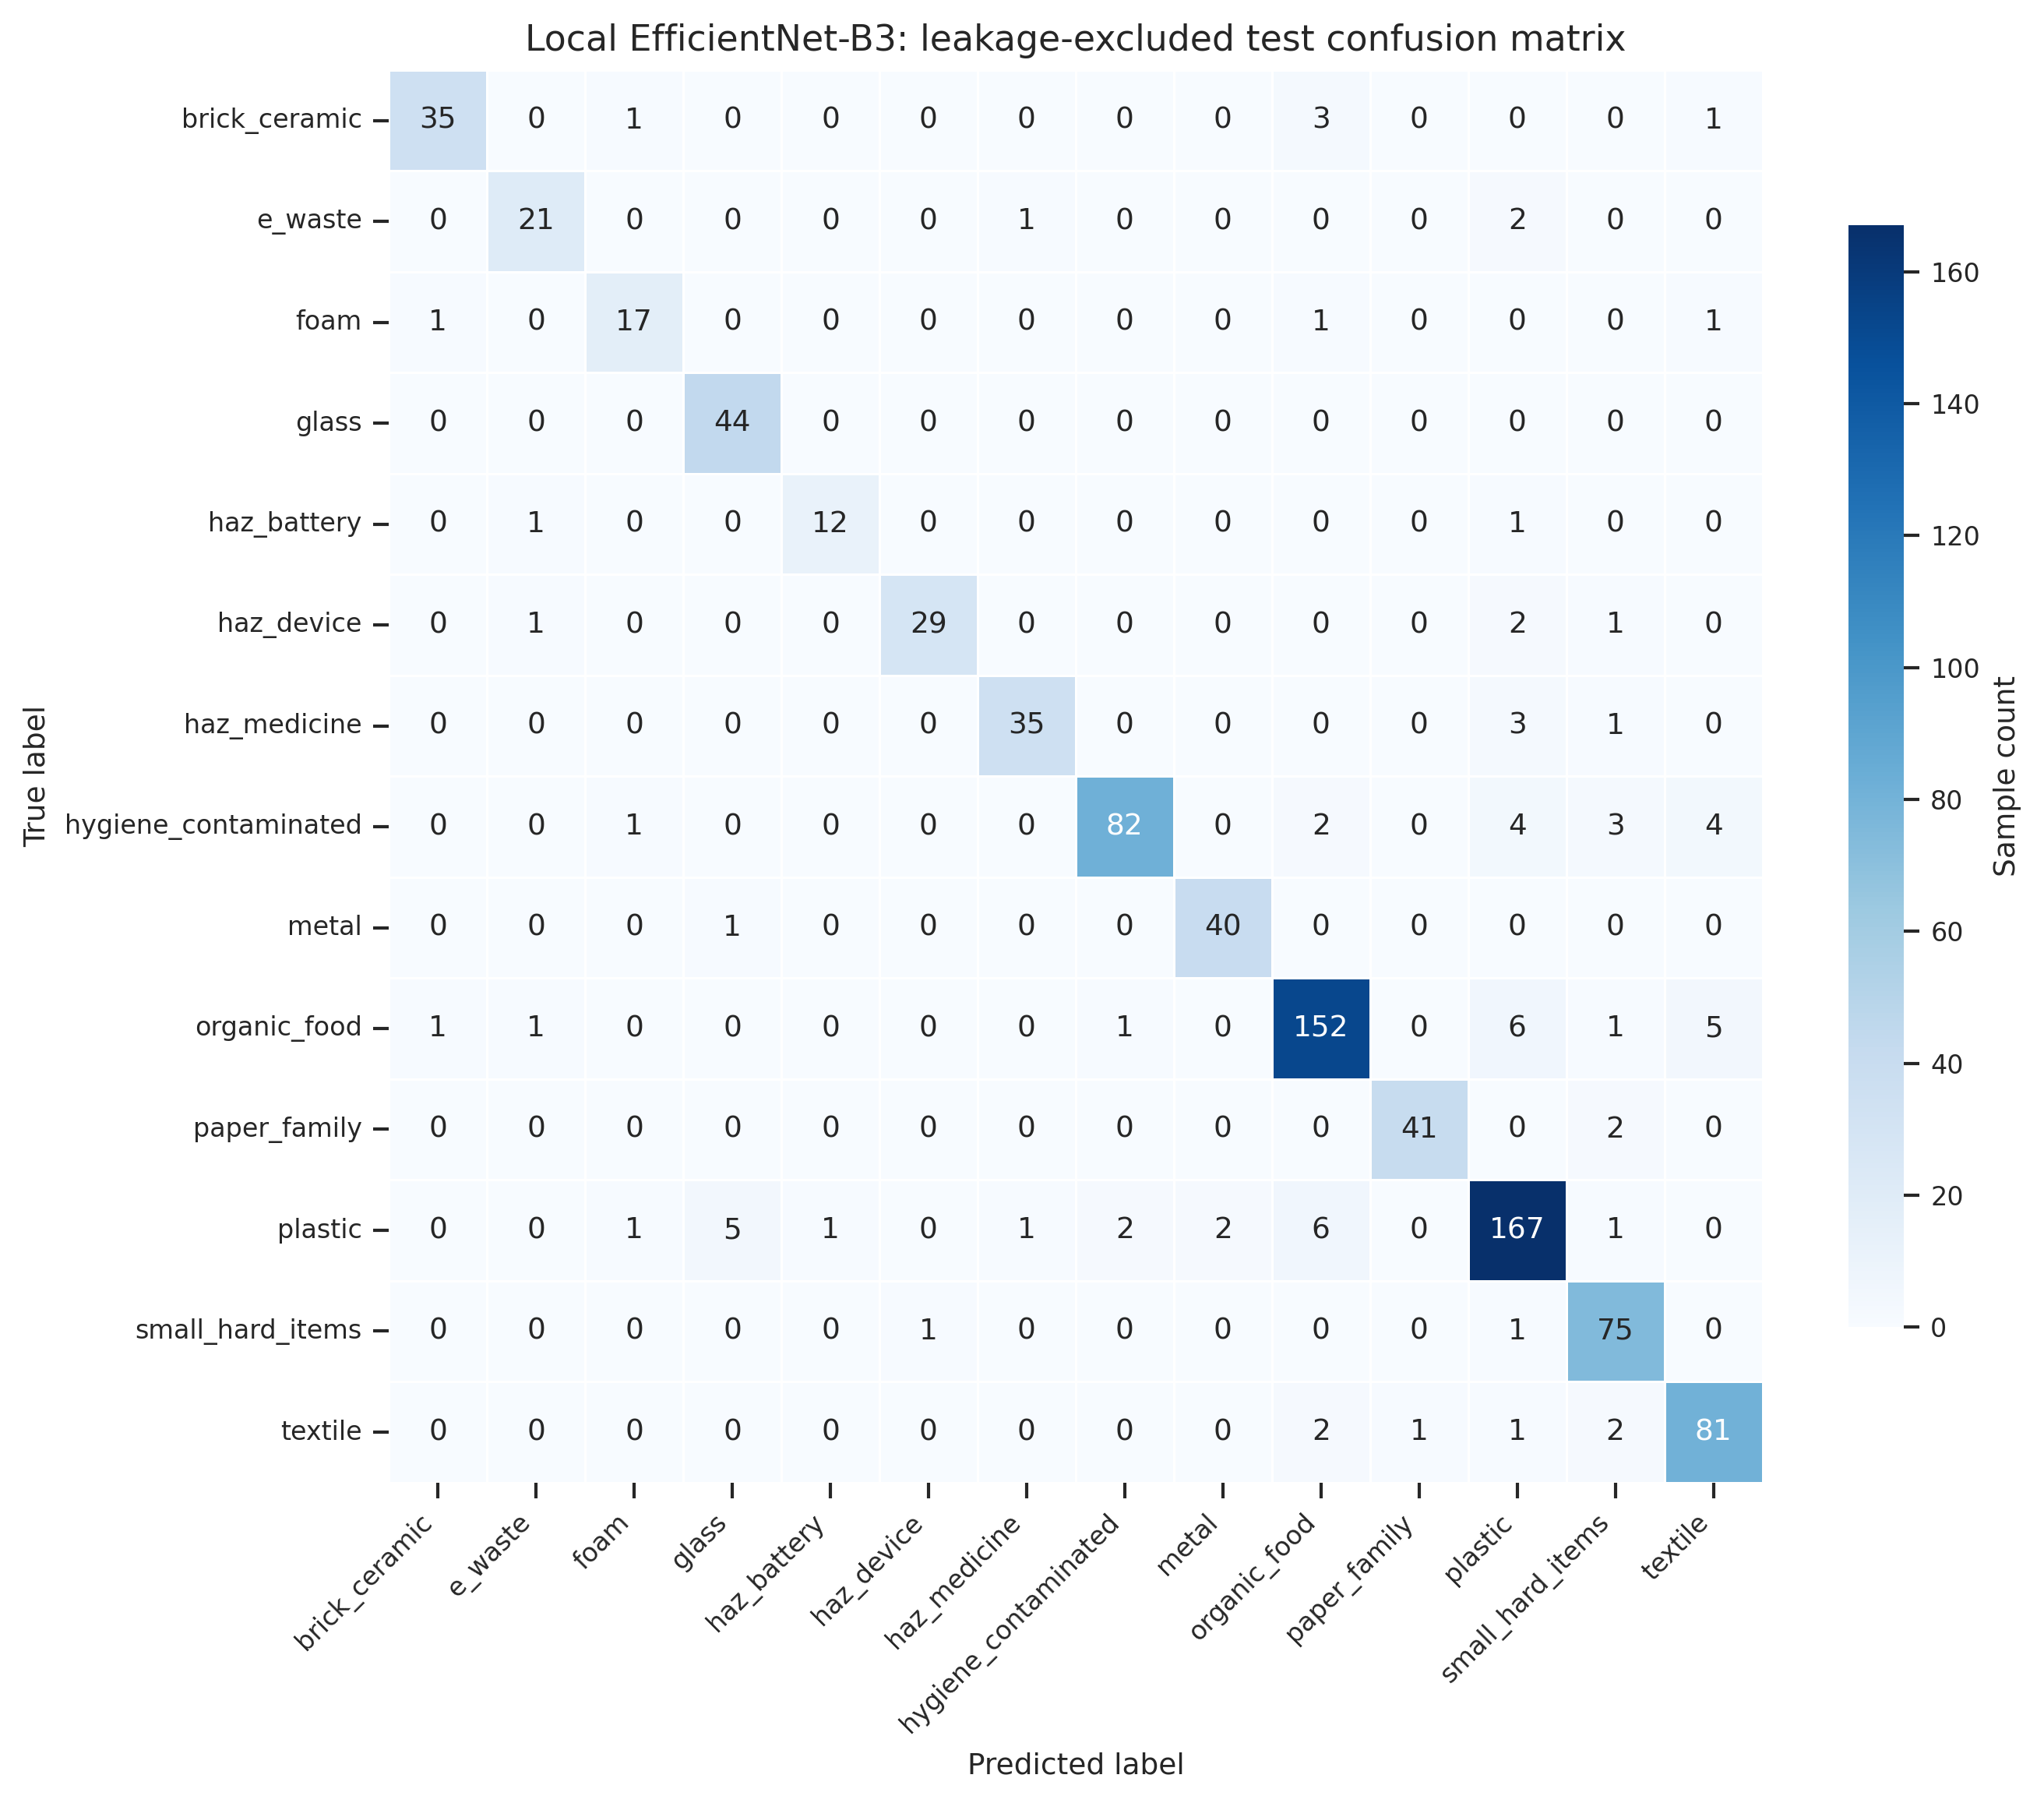
\includegraphics{ecosort_experiment_results/analysis/baseline_confusion_matrix.png}

最大无向混淆对为 \texttt{organic\_food\ ↔\ plastic}，共 12
个，占全部错误 15.0\%。随后是 \texttt{organic\_food\ ↔\ textile} 7
个、\texttt{hygiene\_contaminated\ ↔\ plastic} 6
个、\texttt{plastic\ →\ glass} 5 个。前四组共 30/80，占 37.5\%。

\hypertarget{34-ux6bcfux7c7bux6307ux6807}{%
\subsubsection{3.4 每类指标}\label{34-ux6bcfux7c7bux6307ux6807}}

\begingroup
\small
\setlength{\tabcolsep}{3pt}
\begin{longtable}[]{@{}lrrrr@{}}
\toprule
Class & Precision & Recall & F1 & Support \\
\midrule
\endhead
brick\_ceramic & 94.59\% & 87.50\% & 90.91\% & 40 \\
e\_waste & 87.50\% & 87.50\% & 87.50\% & 24 \\
foam & 85.00\% & 85.00\% & 85.00\% & 20 \\
glass & 88.00\% & 100.00\% & 93.62\% & 44 \\
haz\_battery & 92.31\% & 85.71\% & 88.89\% & 14 \\
haz\_device & 96.67\% & 87.88\% & 92.06\% & 33 \\
haz\_medicine & 94.59\% & 89.74\% & 92.11\% & 39 \\
hygiene\_contaminated & 96.47\% & 85.42\% & 90.61\% & 96 \\
metal & 95.24\% & 97.56\% & 96.39\% & 41 \\
organic\_food & 91.57\% & 91.02\% & 91.29\% & 167 \\
paper\_family & 97.62\% & 95.35\% & 96.47\% & 43 \\
plastic & 89.30\% & 89.78\% & 89.54\% & 186 \\
small\_hard\_items & 87.21\% & 97.40\% & 92.02\% & 77 \\
textile & 88.04\% & 93.10\% & 90.50\% & 87 \\
\bottomrule
\end{longtable}
\endgroup

\hypertarget{4-uncertainty-routing}{%
\subsection{4. Uncertainty Routing}\label{4-uncertainty-routing}}

\hypertarget{41-ux5ba1ux8ba1ux5230ux7684ux73b0ux6709ux6307ux6807}{%
\subsubsection{4.1
审计到的现有指标}\label{41-ux5ba1ux8ba1ux5230ux7684ux73b0ux6709ux6307ux6807}}

本轮没有添加新的 uncertainty 指标，只复现现有 Streamlit strict threshold
公式：

\begin{itemize}
\tightlist
\item
  Top-1 Confidence：\texttt{max(p)}；低于阈值时拒绝。
\item
  Top1--Top2 Margin：最高与次高概率差；低于阈值时拒绝。
\item
  Normalized
  Entropy：\texttt{−Σ\ p\ log\ p\ /\ log(K)}；高于阈值时拒绝。
\item
  Hazardous-class guard：预测为危险类且置信度低于特殊阈值时拒绝。
\end{itemize}

现有实现存在三个事实差异。根 \texttt{backend/app.py} 的产品推理只用
\texttt{confidence\ \textless{}\ 0.7} 并由用户手动触发 AI review；完整
Confidence + Margin + Entropy + Hazard guard 位于
\texttt{streamlit\_demo.py}，但只返回 review-needed，不自动调用
VLM。后者的 hazardous 集合仍是旧标签，V6 14 类中只有 \texttt{e\_waste}
能命中，\texttt{haz\_battery\ /\ haz\_device\ /\ haz\_medicine}
均不会命中。此外，Streamlit 实际使用 300×300 直接
Resize、CPU/FP32，而本实验使用 checkpoint 对应的 224 letterbox、L20
FP16；因此下文 \texttt{Current\ full} 表示``Streamlit
阈值逻辑施加于标准化 checkpoint 输出''，不是当前 Streamlit 端到端行为。

\hypertarget{42-ad-ablationux56faux5b9aux9ed8ux8ba4ux9608ux503ctest}{%
\subsubsection{4.2 A--D
Ablation（固定默认阈值，Test）}\label{42-ad-ablationux56faux5b9aux9ed8ux8ba4ux9608ux503ctest}}

\begingroup
\small
\setlength{\tabcolsep}{3pt}
\begin{longtable}[]{@{}lrrrrrrr@{}}
\toprule
Strategy & Coverage & Route rate & Errors caught & Acc\_sel & F1\_sel &
ED-Precision & ED-Recall \\
\midrule
\endhead
A. Confidence & 84.413\% & 15.587\% & 56 / 80 & 96.879\% & 96.783\% &
39.437\% & 70.000\% \\
B. + Margin & 84.413\% & 15.587\% & 56 / 80 & 96.879\% & 96.783\% &
39.437\% & 70.000\% \\
C. + Entropy & 84.413\% & 15.587\% & 56 / 80 & 96.879\% & 96.783\% &
39.437\% & 70.000\% \\
D. Current full & 84.303\% & 15.697\% & 56 / 80 & 96.875\% & 96.754\% &
39.161\% & 70.000\% \\
\bottomrule
\end{longtable}
\endgroup

拒绝本身不产生替代预测，因此表中的 Accepted Acc / Macro-F1
只描述被本地模型接受的子集，不能当作系统 Overall
指标。若仍保留被拒样本的原本地预测，则 Overall Accuracy / Macro-F1 仍是
91.218\% / 91.208\%。

A、B、C 的决策完全相同，说明在当前默认阈值和当前预测分布上，Margin 与
Entropy 没有提供 Confidence 之外的增量。D 只多拒绝一个预测正确的
\texttt{e\_waste}，没有多捕获错误。当前最简洁的 operating strategy
因而是 A，而不是完整 D。

\hypertarget{43-threshold-sweepconfidence-only}{%
\subsubsection{4.3 Threshold
Sweep（Confidence-only）}\label{43-threshold-sweepconfidence-only}}

阈值候选在排除确认精确重复的 validation（N=895）上选择，再一次性应用到
test；没有根据 test 结果反向调阈值。

\begingroup
\small
\setlength{\tabcolsep}{3pt}
\begin{longtable}[]{@{}rrrrrrr@{}}
\toprule
Threshold & Coverage & Route rate & Acc\_sel & F1\_sel & ED-Precision &
ED-Recall \\
\midrule
\endhead
0.50 & 98.024\% & 1.976\% & 92.497\% & 92.967\% & 72.222\% & 16.250\% \\
0.55 & 96.817\% & 3.183\% & 92.971\% & 93.232\% & 62.069\% & 22.500\% \\
0.60 & 94.841\% & 5.159\% & 93.866\% & 94.159\% & 57.447\% & 33.750\% \\
0.65 & 93.524\% & 6.476\% & 94.249\% & 94.478\% & 52.542\% & 38.750\% \\
0.70 & 91.877\% & 8.123\% & 94.624\% & 94.886\% & 47.297\% & 43.750\% \\
0.75 & 90.011\% & 9.989\% & 94.878\% & 95.122\% & 41.758\% & 47.500\% \\
0.80 & 87.925\% & 12.075\% & 95.880\% & 96.090\% & 42.727\% &
58.750\% \\
\textbf{0.85} & \textbf{84.413\%} & \textbf{15.587\%} &
\textbf{96.879\%} & \textbf{96.783\%} & \textbf{39.437\%} &
\textbf{70.000\%} \\
0.90 & 79.912\% & 20.088\% & 97.253\% & 96.992\% & 32.787\% &
75.000\% \\
0.95 & 66.850\% & 33.150\% & 98.358\% & 98.395\% & 23.179\% &
87.500\% \\
\bottomrule
\end{longtable}
\endgroup

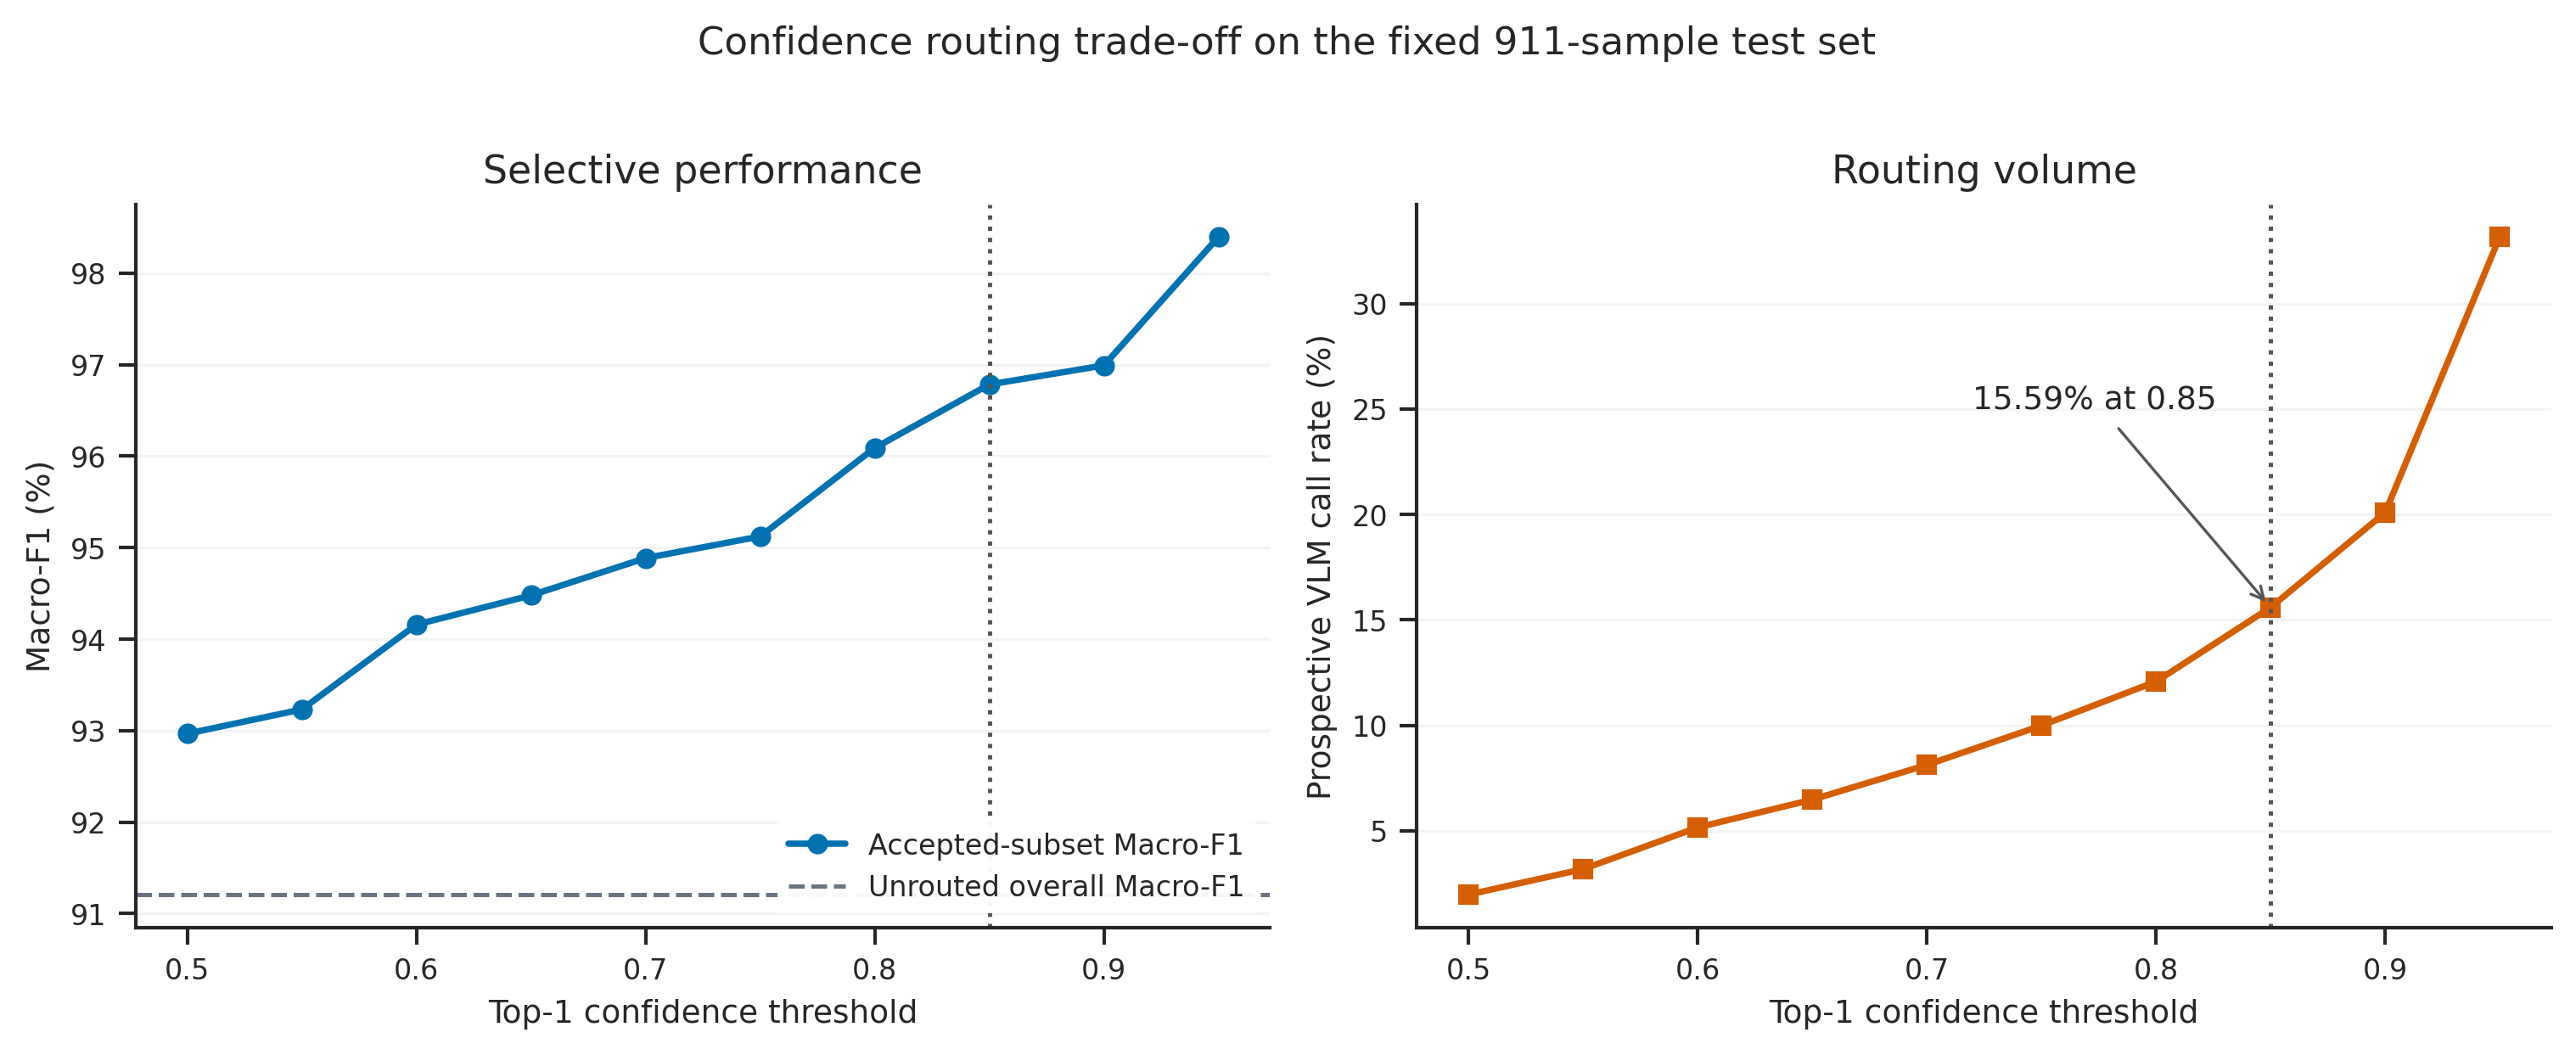
\includegraphics{ecosort_experiment_results/analysis/threshold_tradeoff.png}

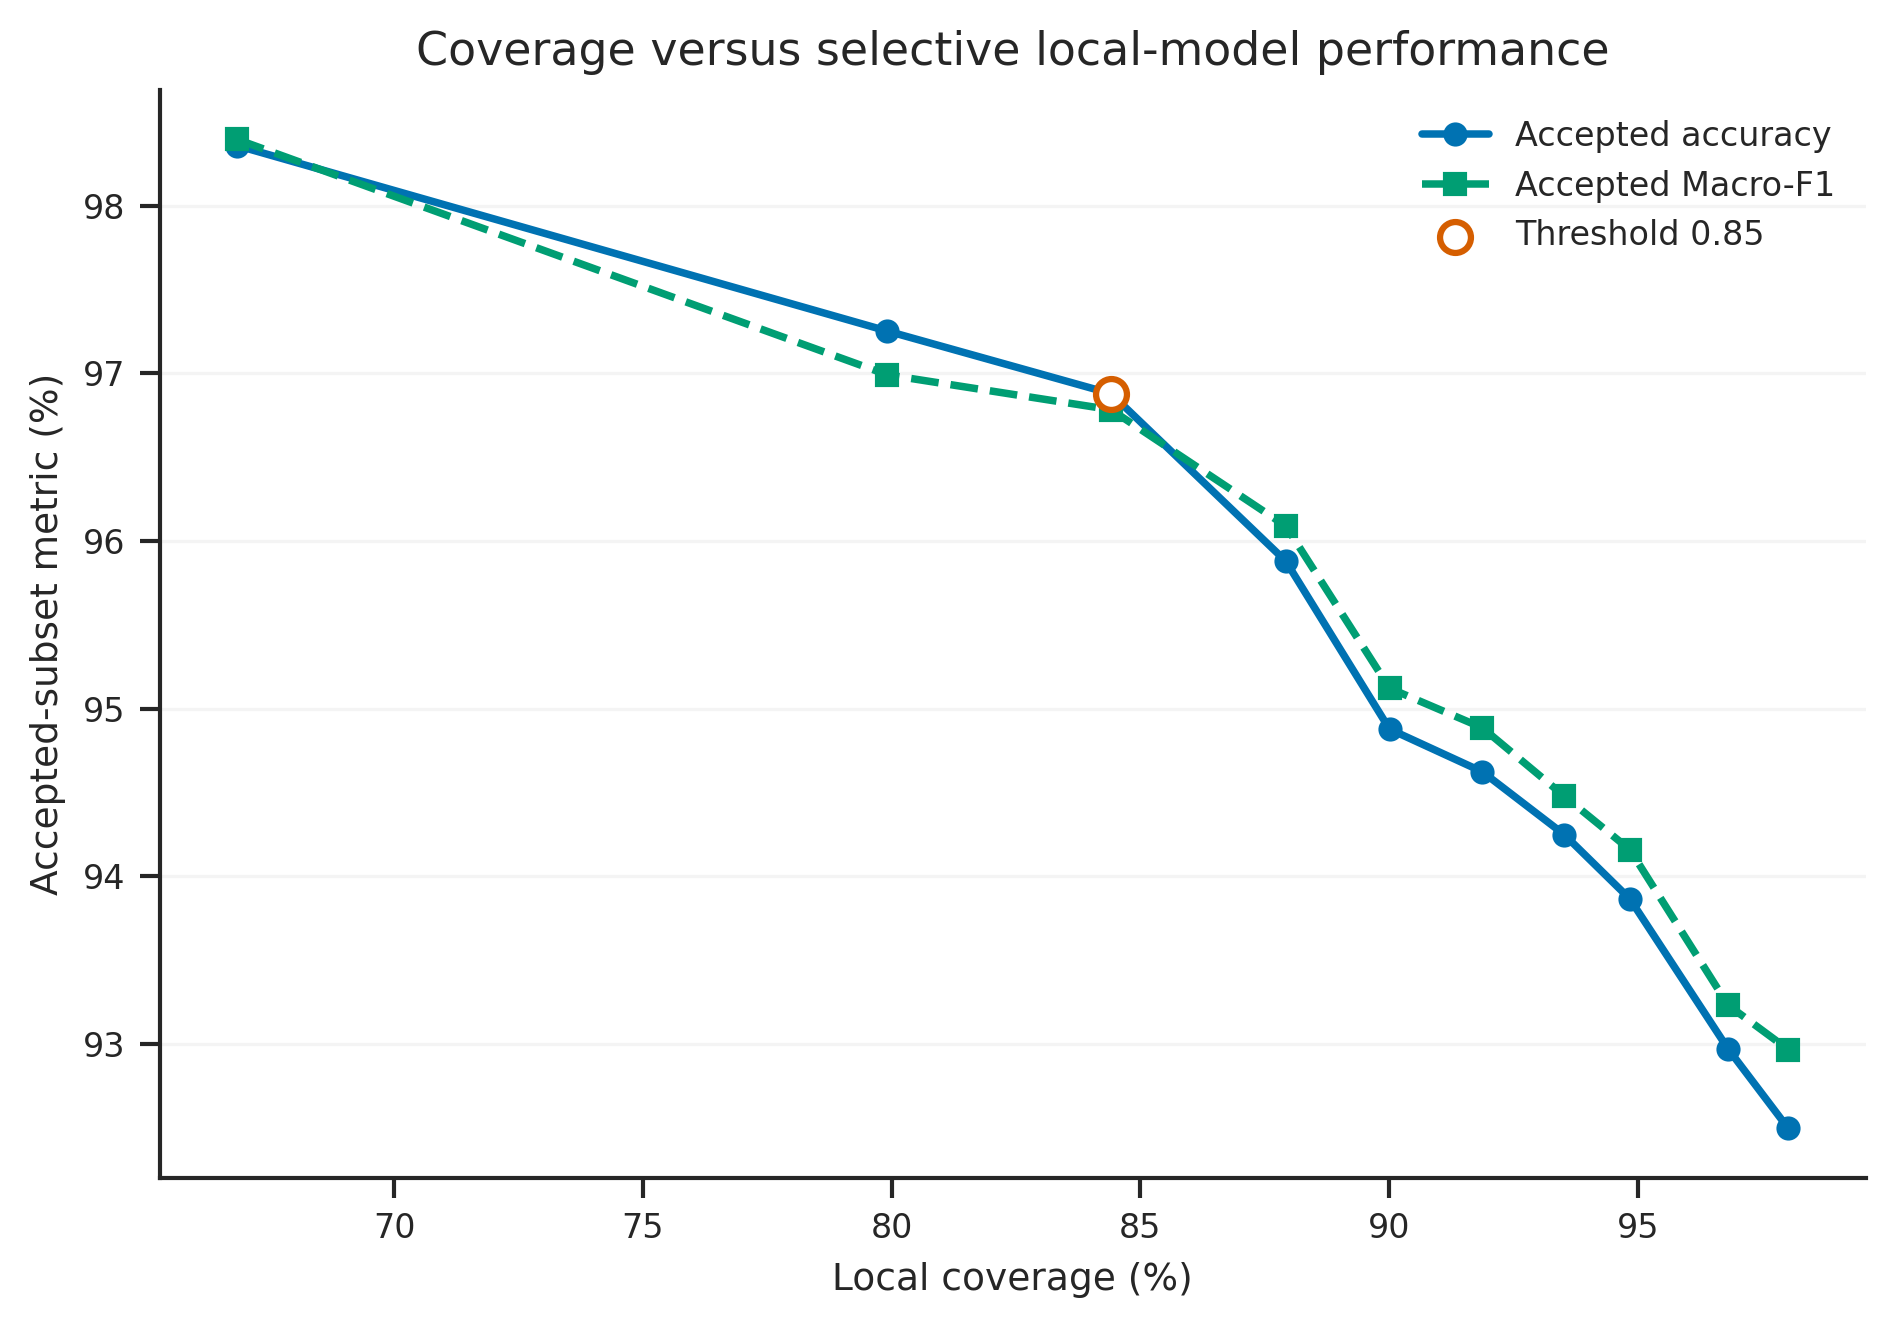
\includegraphics{ecosort_experiment_results/analysis/coverage_vs_accuracy.png}

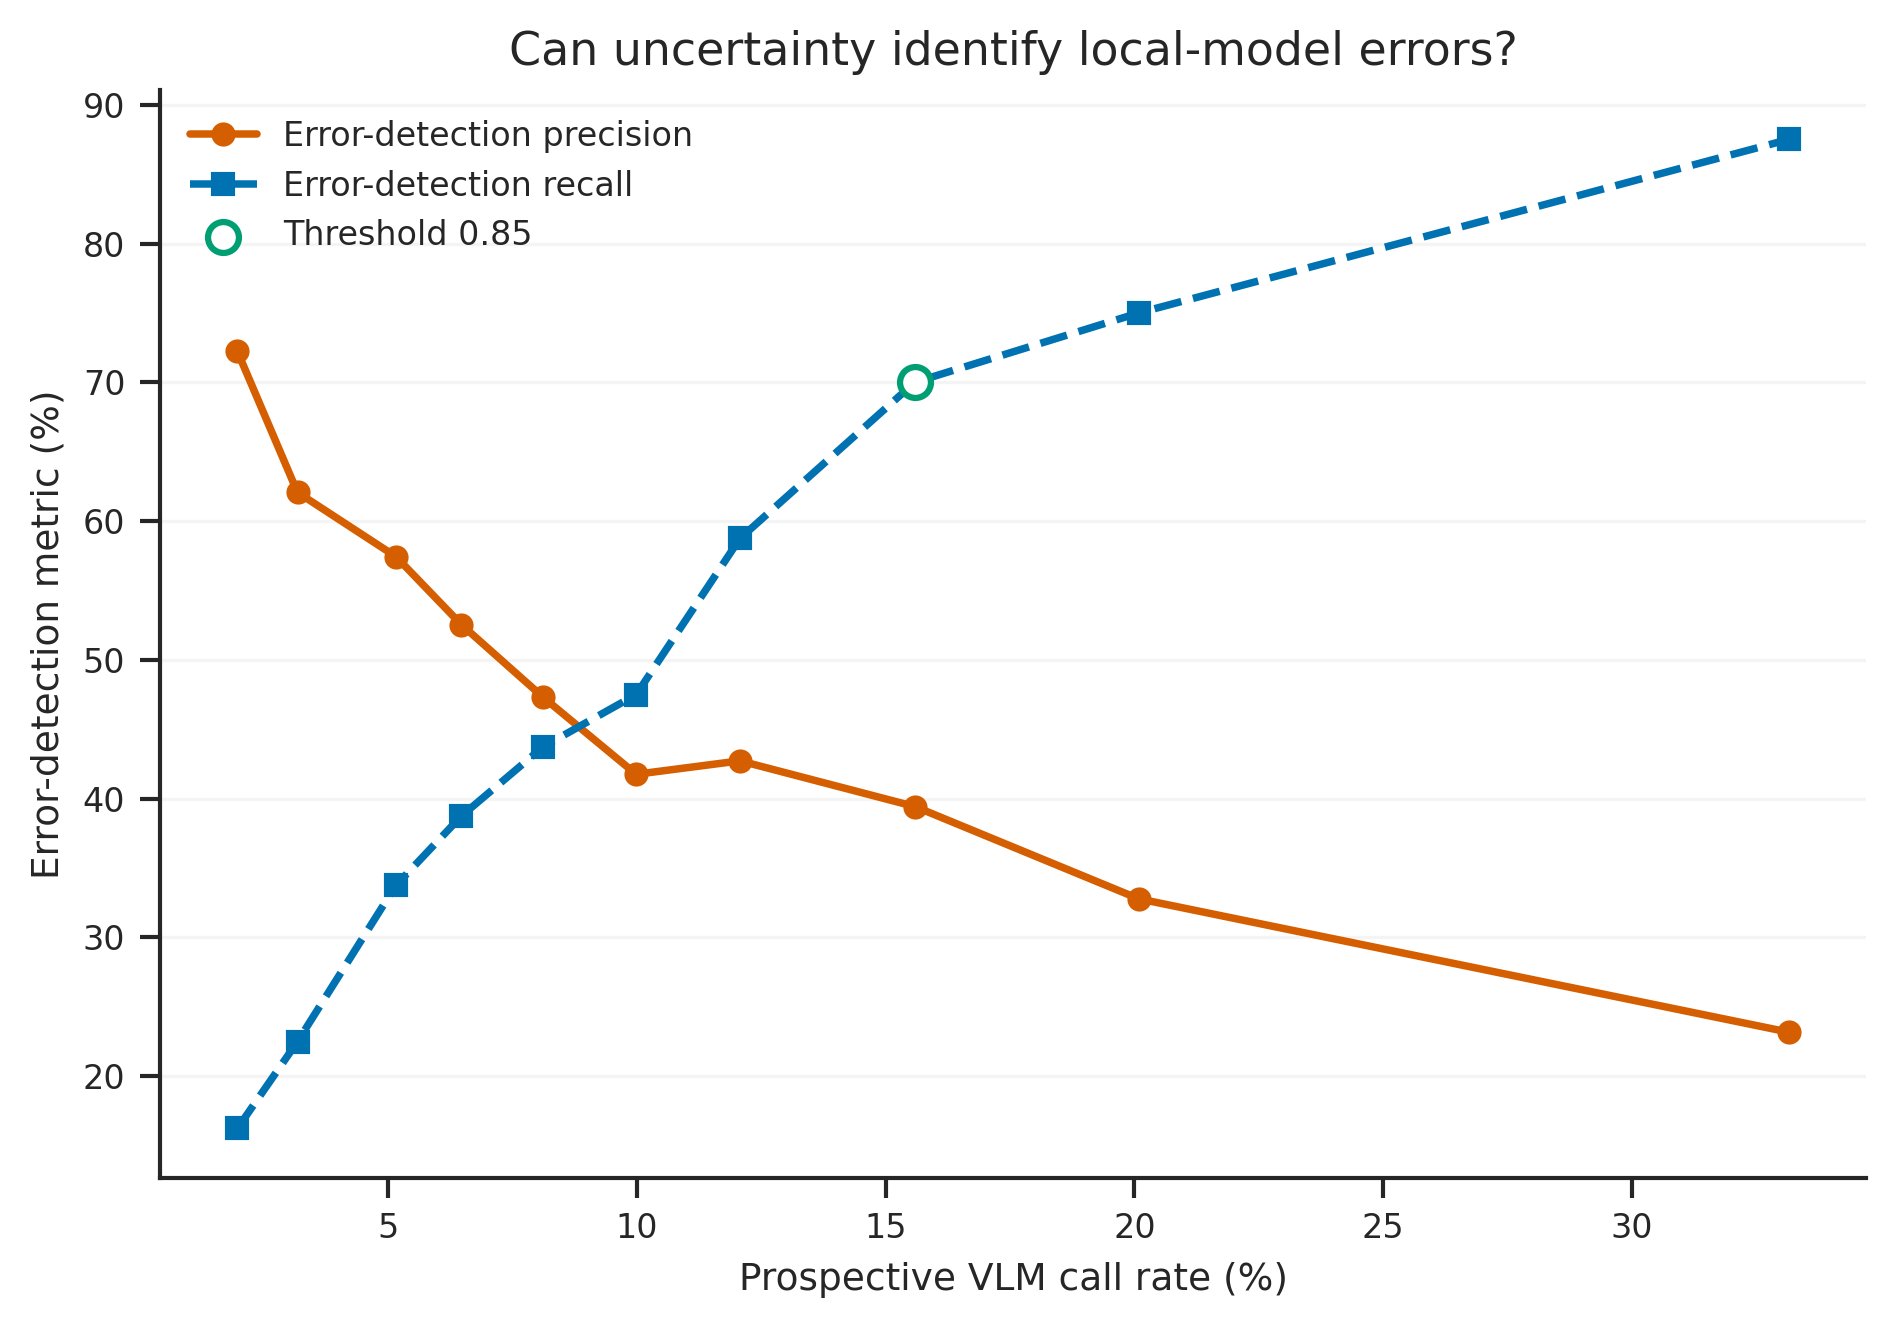
\includegraphics{ecosort_experiment_results/analysis/error_detection_tradeoff.png}

\hypertarget{44-operating-point}{%
\subsubsection{4.4 Operating Point}\label{44-operating-point}}

建议的路由 operating point 是 \textbf{Confidence-only，threshold=0.85}。

\begin{itemize}
\tightlist
\item
  Validation：路由 110/895（12.291\%），错误检测 Recall
  69.811\%，Precision 33.636\%。
\item
  Test：路由 142/911（15.587\%），错误检测 Recall 70.000\%，Precision
  39.437\%，错误检测 F1 50.450\%。
\item
  相比 0.90，0.85 少约 4.5 个百分点的预期调用量，只少捕获 4/80
  个本地错误；相比 0.75，则多约 5.6 个百分点调用量并多捕获 18/80
  个错误。
\end{itemize}

这个点证明路由有筛错能力，但不证明被路由样本一定能被 VLM 修正。

\hypertarget{5-vlm-cascade}{%
\subsection{5. VLM Cascade}\label{5-vlm-cascade}}

\hypertarget{51-ux73b0ux6709ux5b9eux73b0ux4e0eux590dux7528ux8fb9ux754c}{%
\subsubsection{5.1
现有实现与复用边界}\label{51-ux73b0ux6709ux5b9eux73b0ux4e0eux590dux7528ux8fb9ux754c}}

根 \texttt{backend/app.py} 定义了现有 42 类 VLM
任务。本轮保持该任务语义和 \texttt{configs/dataset\_mapping.yaml}
不变，仅把真实 provider 固定为 \texttt{doubao-seed-2-0-lite-260428}。41
个原始类可映射到 V6 14 类；唯一无映射输出是已从 V6 删除的
\texttt{trash}。公平评测只采用 VLM Top-1；非法输出、\texttt{trash} 或
API 错误标记为 failure，最终保留 local 预测。

\texttt{delivery/clean\_github\_upload} 是 V5 部署快照，自动 fallback
只输出 4 个粗类，不能用于本轮 14 类 Macro-F1；HF Space 也明确不调用云
VLM。因此没有把旧部署结果冒充为 V6 cascade。

此前 Gemini 试运行因免费限额中止且样本不完整，其 cache 保留在独立目录
\texttt{reports/ecosort\_experiment\_results/vlm}，不参与本轮
Seed2.0-Lite 正式结果。

\hypertarget{52-ux5b89ux5168ux8c03ux7528ux8ba1ux5212}{%
\subsubsection{5.2
安全调用计划}\label{52-ux5b89ux5168ux8c03ux7528ux8ba1ux5212}}

固定调用计划采用已选定的 Confidence-only
\texttt{confidence\ \textless{}\ 0.85}：142/911（15.587\%）。独立 Seed
harness 具备：

\begin{itemize}
\tightlist
\item
  默认 dry-run，必须显式 \texttt{-\/-execute} 才会请求外部 API；
\item
  结果 cache 与永久预算账本分离；model、prompt、mapping
  或图像变化只会使结果不可复用，不会返还已消耗预算；
\item
  每次请求前先在独占文件锁内写入带 \texttt{attempt\_id} 的 reservation
  并 \texttt{fsync}；在固定默认 output directory
  且不删除账本的前提下，所有并发进程共享累计 142 次 generation-attempt
  上限；
\item
  若进程在请求后崩溃，未完成 reservation
  会保守占用额度且禁止自动重试，从而避免重复收费；显式重试也只能消耗剩余累计预算；
\item
  cache key 包含 sample ID、图像 SHA256、model、helper 源码 hash
  和映射文件 hash；
\item
  每次返回结果单独写入 JSONL + flush + fsync，支持中断恢复；
\item
  单次 wall timeout 120 秒；
\item
  通过受保护文件读取 key，\texttt{requests.Session(trust\_env=False)}
  避免代理污染，key 不写入结果文件或日志。
\end{itemize}

执行状态：先完成 1-call smoke，再断点续跑其余 141 个样本；最终
ledger=142、cache=142、悬空 reservation=0。140 次成功映射；1 次返回
\texttt{trash} 无法映射，1 次因图像超过 Ark 输入限制返回 HTTP
400，两者均保留原 local 预测且未重试。

\hypertarget{53-cascade-ux7ed3ux679cux72b6ux6001}{%
\subsubsection{5.3 Cascade
结果状态}\label{53-cascade-ux7ed3ux679cux72b6ux6001}}

\begingroup
\small
\setlength{\tabcolsep}{3pt}
\begin{longtable}[]{@{}lrrrrrr@{}}
\toprule
Method & Acc & Macro-P & Macro-R & Macro-F1 & VLM rate & P95 \\
\midrule
\endhead
Local EfficientNet-B3 & 91.218\% & 91.723\% & 90.927\% & 91.208\% & 0\%
& 65.6 ms \\
+ Seed cascade & \textbf{96.158\%} & \textbf{96.744\%} &
\textbf{96.117\%} & \textbf{96.337\%} & \textbf{15.587\%} &
\textbf{4.140 s} \\
\bottomrule
\end{longtable}
\endgroup

142 个 routed 样本中原有 56 个 local error。VLM 修正 49 个、未修正 7
个；86 个原本正确样本中 4 个被改错，Net
Corrected=45。公开机器结果统一收录于
\href{../docs/portfolio/data/summary.json}{summary.json}。

\hypertarget{54-ux914dux5bf9ux7edfux8ba1ux7a33ux5065ux6027}{%
\subsubsection{5.4
配对统计稳健性}\label{54-ux914dux5bf9ux7edfux8ba1ux7a33ux5065ux6027}}

在不改变模型、路由阈值或任何逐样本预测的前提下，对 911 个成对的
Local/Cascade 结果进行 10,000 次样本级 paired
bootstrap（seed=20260811），并对正确性变化执行 exact McNemar test。

\begingroup
\small
\setlength{\tabcolsep}{3pt}
\begin{longtable}[]{@{}lrr@{}}
\toprule
Paired delta & Point estimate & Bootstrap 95\% CI \\
\midrule
\endhead
Accuracy & +4.940 pp & {[}+3.403, +6.476{]} pp \\
Macro Precision & +5.021 pp & {[}+2.912, +7.346{]} pp \\
Macro Recall & +5.190 pp & {[}+3.235, +7.448{]} pp \\
Macro-F1 & \textbf{+5.129 pp} & \textbf{{[}+3.328, +7.275{]} pp} \\
\bottomrule
\end{longtable}
\endgroup

53 个 Local 与 Cascade 结果不一致的样本中，49 个是 Local wrong→Cascade
correct，4 个是 Local correct→Cascade wrong；exact McNemar 双侧
\texttt{p=7.054e-11}。在 142 个 routed 样本内部，Accuracy 从 60.563\%
提升至 92.254\%（+31.690
pp）。因此，固定测试集上的净提升具有明确配对统计证据，不是由少数随机翻转即可解释。

置信区间只量化该固定测试集的抽样不确定性，不覆盖标签噪声、阈值选择、数据分布漂移、VLM
provider/version 漂移或未来网络状态。逐类分析显示 14 类中 13
类点估计提高，但 \texttt{paper\_family} F1 下降 5.166 pp，主要因为部分
\texttt{tissue} 图像被 VLM 视觉合理地判为纸类却与目录映射标签冲突。

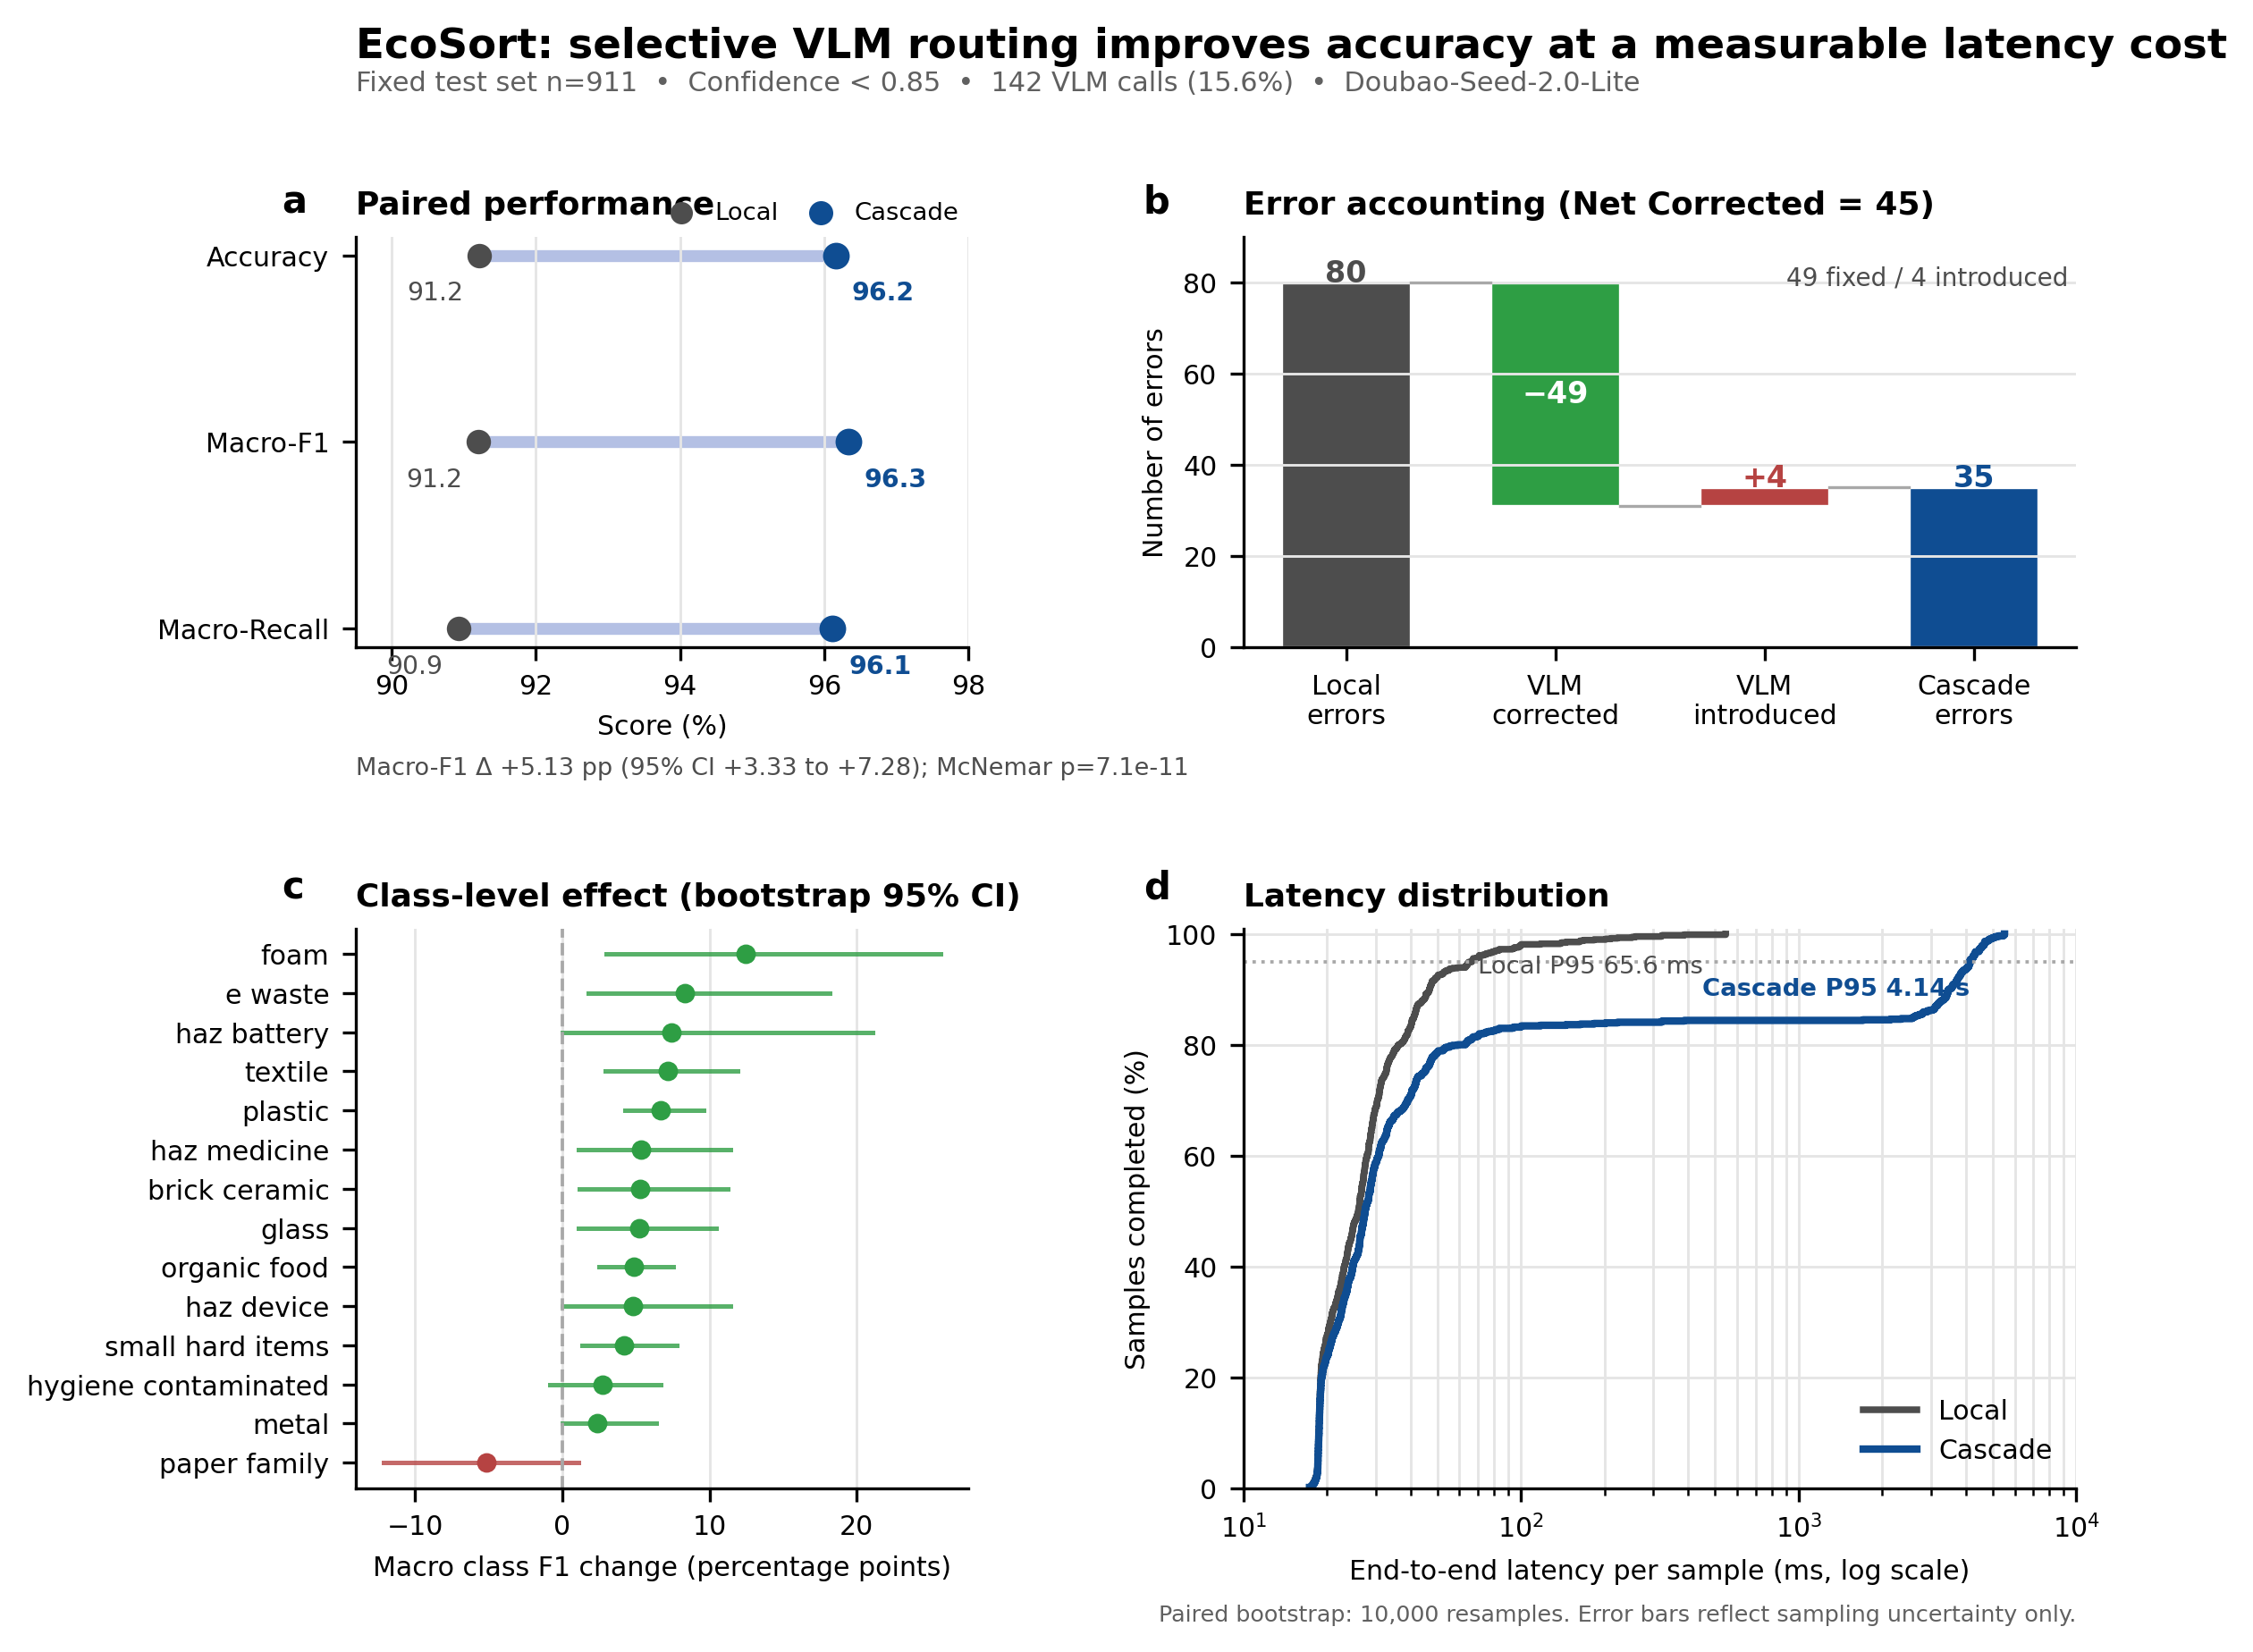
\includegraphics{../docs/portfolio/assets/ecosort_cascade_summary.png}

公开机器结果：\href{../docs/portfolio/data/summary.json}{summary.json}、\href{../docs/portfolio/data/per_class_delta.csv}{per\_class\_delta.csv}。10,000
次逐次 bootstrap
明细保留在本地审计目录，公开包提供点估计、置信区间和生成代码。

\hypertarget{6-metrics--latency}{%
\subsection{6. Metrics / Latency}\label{6-metrics--latency}}

本地延迟以单样本、batch=1、L20、FP16、20 次 warmup 计量；每个样本都做
CUDA synchronize。Forward latency 从 H2D 完成后计至 softmax
与同步；End-to-end 包含 PIL 解码、letterbox、H2D、forward、softmax
和后处理。

\begingroup
\small
\setlength{\tabcolsep}{3pt}
\begin{longtable}[]{@{}lrrr@{}}
\toprule
Latency scope & Mean & P50 & P95 \\
\midrule
\endhead
Forward & 16.319 ms & 15.472 ms & 16.134 ms \\
End-to-end & 32.808 ms & 25.977 ms & 65.621 ms \\
\bottomrule
\end{longtable}
\endgroup

本地数字不包含网络 VLM。真实调用 harness 在图像解码/转换完成后开始 VLM
request timer，并把 request wall time 与已含一次解码的 local end-to-end
相加。全 911 样本的最终 Cascade Mean/P50/P95 分别为
618.600/27.444/4,139.525 ms；仅 142 个 routed 请求的 VLM latency
Mean/P50/P95 分别为 3,758.150/3,739.919/4,926.170 ms。

\hypertarget{7-ablation}{%
\subsection{7. Ablation}\label{7-ablation}}

A--D
消融的关键事实不是``指标越堆越好''，而是三个指标在当前概率分布上高度冗余：A、B、C
的 142 个拒绝样本完全相同；D 的 hazardous guard
因标签集合过时只多拒绝一个正确样本。此结果支持简化到
Confidence-only，而不是为简历保留没有增量的 Margin/Entropy 组合。

这不表示 Margin 或 Entropy 在所有模型上都无效，只表示它们在当前
checkpoint、当前阈值与当前测试分布上没有可测增量。

\hypertarget{8-threshold-trade-off}{%
\subsection{8. Threshold Trade-off}\label{8-threshold-trade-off}}

阈值提高会提高 accepted-subset Accuracy / Macro-F1 和错误检测
Recall，但同时快速降低 local coverage、降低错误检测 Precision。0.85
位于一个有实际解释的中间区域：只把约六分之一样本列为候选，就捕获 70\%
本地错误；继续升到 0.90 仅多捕获 5 个百分点错误，却将候选调用量提升到
20.09\%。

这里的``候选调用量''仍是 prospective call rate。只有实际 VLM
结果完成后，才能把横轴升级为真实成本，把纵轴升级为 cascade Overall
Accuracy / Macro-F1。

\hypertarget{9-latency--call-rate}{%
\subsection{9. Latency / Call Rate}\label{9-latency--call-rate}}

建议分别报告三种量，避免混淆：

\begin{enumerate}
\def\labelenumi{\arabic{enumi}.}
\tightlist
\item
  Local coverage：本地模型直接接受比例；0.85 时为 84.413\%。
\item
  Prospective VLM rate：按固定 Confidence-only 规则应调用比例，为
  15.587\%。
\item
  Actual VLM rate：真实 API attempts / 911，为 142/911=15.587\%；成功
  140，失败 2。
\end{enumerate}

141 次响应返回 usage，合计 input 231,211、output 15,102、total 246,313
tokens；HTTP 400 的 1 次请求没有 usage
metadata。没有真实价格配置，因此不报告货币成本。

\hypertarget{10-bad-cases}{%
\subsection{10. Bad Cases}\label{10-bad-cases}}

\hypertarget{101-ux8defux7531ux7b5bux9519ux80fdux529b}{%
\subsubsection{10.1
路由筛错能力}\label{101-ux8defux7531ux7b5bux9519ux80fdux529b}}

在 80 个本地错误中，\texttt{confidence\ \textless{}\ 0.85} 捕获 56
个；同时误拒 86 个原本预测正确的样本。因此 error-detection Precision
只有 39.437\%。仍有 24 个 confident-but-wrong，占全部错误 30\%；其中 20
个 confidence≥0.90，10 个≥0.95。

24 个高置信错误的平均 Confidence=0.9405、Margin=0.9137、Normalized
Entropy=0.1211，真实类别只有 11/24 位于
Top-2。它们在三个现有信号上都表现得非常确定，单纯微调 Confidence /
Margin / Entropy 无法全部识别。

\hypertarget{102-ux4ee3ux8868ux6027ux6837ux672c}{%
\subsubsection{10.2
代表性样本}\label{102-ux4ee3ux8868ux6027ux6837ux672c}}

\begin{itemize}
\tightlist
\item
  \texttt{organic\_food\_000029.jpg}：organic\_food →
  plastic，confidence=0.9956。混合垃圾堆占主体，花只在前景；目录
  \texttt{flower→organic\_food} 与画面主体不一致。
\item
  \texttt{plastic\_000181.jpg}：plastic →
  organic\_food，confidence=0.9706。鸭形玩具视觉上更像木制品，\texttt{plastic\_toy→plastic}
  疑似目录级标签噪声。
\item
  \texttt{foam\_000010.jpg}：foam →
  brick\_ceramic，confidence=0.9783。刚性多孔白块在纹理和形态上接近陶瓷/砖材。
\item
  \texttt{hygiene\_contaminated\_000074.jpg}：hygiene\_contaminated →
  small\_hard\_items，confidence=0.9739。烟头的处置语义与细长硬物外观冲突。
\item
  \texttt{haz\_device\_000002.jpg}：haz\_device →
  e\_waste，confidence=0.9521。灯泡式电子物体同时符合两类语义边界。
\item
  \texttt{paper\_family\_000002.jpg}：paper\_family →
  small\_hard\_items，confidence=0.9298。报纸主体清楚，属于真实模型/校准错误。
\end{itemize}

\hypertarget{103-ux74f6ux9888ux5f52ux56e0}{%
\subsubsection{10.3 瓶颈归因}\label{103-ux74f6ux9888ux5f52ux56e0}}

\begin{enumerate}
\def\labelenumi{\arabic{enumi}.}
\tightlist
\item
  \textbf{当前定向人工审查显示，数据质量与类别定义是主要结构性风险。}
  标签由原始目录整体映射，如
  \texttt{plastic\_toy→plastic}、\texttt{bag→textile}、\texttt{flower/tea/bone→organic\_food}、\texttt{lighter→haz\_medicine}，单图材质未逐一核验；由于只人工审查了
  12 个代表样本，尚不能据此对全部 80 个错误的瓶颈占比作严格排序。
\item
  \textbf{本地模型仍有真实视觉与上下文偏置。}
  报纸、电池、LEGO、陶瓷盘等清晰目标仍出现高置信错误；背景垃圾、污渍和容器材质会压过主体语义。
\item
  \textbf{Uncertainty calibration 有效但不充分。} 70\% 错误召回与 39.4\%
  精度说明路由有筛错价值，也会产生大量误拒；24
  个高置信错误无法由当前三项信号发现。
\item
  \textbf{VLM 对对象功能语义有明确价值，但受项目标签边界约束。}
  它修正了电池/电子垃圾、药品/塑料等多类错误；同时
  \texttt{tissue→hygiene\_contaminated}、\texttt{tea→organic\_food}
  等目录映射使部分视觉合理的 VLM 输出仍被计错。
\item
  \textbf{类别不平衡是次要因素。} 测试支持从 14 到 186，相差 13.29
  倍，但小类与大类中都有高、低表现，不能把主要错误简单归因于样本量。
\end{enumerate}

\hypertarget{104-seed-cascade-bad-cases}{%
\subsubsection{10.4 Seed Cascade Bad
Cases}\label{104-seed-cascade-bad-cases}}

四类迁移计数为：\texttt{local\ wrong→VLM\ correct}
49、\texttt{local\ wrong→VLM\ still\ wrong}
7、\texttt{local\ correct→VLM\ correct}
82、\texttt{local\ correct→VLM\ wrong} 4。定向复核全部 7 个未修正样本、4
个新增错误与 2 个 failure 后，得到以下具体结论。

\begin{itemize}
\tightlist
\item
  三个新增错误来自 \texttt{hygiene\_contaminated}：原始 \texttt{tissue}
  目录中的图像实际呈现干净皱纸或废纸，VLM 输出 \texttt{paper\_family}
  在视觉上合理，暴露目录级 \texttt{tissue→hygiene\_contaminated}
  映射噪声。
\item
  \texttt{hygiene\_contaminated\_000007.jpg} 来自 diaper
  目录，但画面只是带食物污渍的白布，VLM 输出
  \texttt{organic\_food}；处置对象和污渍主体不明确。
\item
  \texttt{hygiene\_contaminated\_000037.jpg}
  是未使用的彩色清洁布/湿巾，VLM 输出
  \texttt{textile}；``受污染''属性无法从画面成立。
\item
  \texttt{textile\_000065.jpg} 是大面积脏布纹理，VLM 误判
  \texttt{paper\_family}，属于真实 VLM 材质识别错误，也是 4
  个新增错误之一。
\item
  \texttt{organic\_food\_000122.jpg}
  是茶杯、茶包与包装盒的多对象商品图，VLM 选择
  \texttt{paper\_family}；数据标签按
  \texttt{tea→organic\_food}，主对象定义不一致。
\item
  \texttt{plastic\_000157.jpg} 只拍到深色瓶底，外观像玻璃；local 与 VLM
  均预测 \texttt{glass}，可能是材质视觉歧义或目录标签问题。
\item
  \texttt{organic\_food\_000087.jpg} 来自
  \texttt{flower}，实为混合海洋生物残骸，VLM 输出无映射
  \texttt{trash}，说明 42→14 映射仍有开放集缺口。
\item
  \texttt{plastic\_000027.jpg}
  是含塑料、毛绒、木制和纸箱的混合玩具图，因分辨率超过 Ark 限制返回 HTTP
  400；failure 规则正确保留了原本正确的 local 预测。
\item
  正向样本 \texttt{haz\_battery\_000013.jpg} 中，local 把腐蚀电池盒判为
  \texttt{e\_waste}，VLM 识别电池语义并修正为
  \texttt{haz\_battery}，体现 fallback 在对象功能语义上的价值。
\end{itemize}

公开逐样本结果见
\href{../docs/portfolio/data/routed_transitions.csv}{routed\_transitions.csv}，代表性集合见
\href{../docs/portfolio/data/bad_cases.csv}{bad\_cases.csv}。

\hypertarget{11-limitations}{%
\subsection{11. Limitations}\label{11-limitations}}

\begin{itemize}
\tightlist
\item
  本轮真实验证的是 Doubao-Seed-2.0-Lite 260428、固定 prompt 和固定 0.85
  路由；不能外推到 Gemini、其他 Seed 版本或其他阈值。
\item
  1/142 请求因 Ark 图像尺寸限制失败，1/142 输出 \texttt{trash}
  无法映射；失败保留 local
  能维持系统稳定，但输入预处理和开放集映射仍有工程缺口。
\item
  141/142 请求返回 token
  usage，但没有价格配置，不能从本实验结果推算实际金额。
\item
  结果只覆盖一个 checkpoint、一个固定 14 类 split 和一台
  L20，不能外推到其他硬件或数据分布。
\item
  测试与阈值评估端已排除确认 SHA256 重复，但原 validation 既参与
  champion
  选择，清理后又用于路由阈值校准；残余模型选择泄漏不可回溯量化，且没有独立
  calibration split，operating point 存在适配偏差风险。另有 dHash
  候选可能轻度抬高结果。
\item
  类别规则混合材质、对象功能与处置语义，部分``错误''来自标签边界而非纯视觉识别。
\item
  hazardous guard 仍使用旧标签；Streamlit 的方形 resize 与 champion 的
  224 letterbox 也不一致，产品入口不能直接替代本轮离线评测。
\item
  本轮未做大规模超参数搜索或重训，符合``先回答 cascade
  研究问题''的范围约束。
\end{itemize}

\hypertarget{12-ux6700ux7ec8ux7ed3ux8bba}{%
\subsection{12. 最终结论}\label{12-ux6700ux7ec8ux7ed3ux8bba}}

\hypertarget{ux5df2ux9a8cux8bc1}{%
\subsubsection{已验证}\label{ux5df2ux9a8cux8bc1}}

Local → Uncertainty Estimation → Adaptive Routing → VLM Fallback
的完整链路成立：Confidence-only 0.85 只调用 15.587\% 的 VLM，就把整体
Macro-F1 从 91.208\% 提升至 96.337\%，Accuracy 从 91.218\% 提升至
96.158\%。VLM 修正 49 个错误、引入 4 个错误，净修正 45 个。

\hypertarget{trade-off}{%
\subsubsection{Trade-off}\label{trade-off}}

效果净收益明确，但网络尾延迟也明显：全测试集 P95 从本地 65.621 ms 增至
4.140 s；全测试集 P50 仍为 27.444 ms，因为 84.413\% 样本完全本地处理。该
operating point
适合允许少量困难样本慢路径的异步审核或交互式场景，不适合所有请求都要求亚秒
P95 的同步链路。

\hypertarget{ux662fux5426ux91cdux8bad}{%
\subsubsection{是否重训}\label{ux662fux5426ux91cdux8bad}}

本轮按约束停止，不重训、不调阈值、不修改模型。现有结果已经足以回答
cascade 研究问题。完整复现命令与安全约束见
\url{EXPERIMENT_REPRO.md}，公开机器结果位于
\href{../docs/portfolio/data/}{docs/portfolio/data}；原始账本与 cache
只保留在受控本地审计目录。

\end{document}
